\section{Experiments}
\label{sec:experiments}

\subsection{Experimental Setup}
\label{sec:setup}

\subsubsection{Datasets}

\textbf{Primary Dataset: UCF-Crime}~\cite{sultani2018real}. We use the official test partition (\textbf{290 videos}: 140 anomaly + 150 normal) for all primary results. We additionally report a full-pool evaluation (\textbf{1900 videos}: 950 anomaly + 950 normal, Section~\ref{sec:robustness}) as a separate robustness analysis. It uses only video-level normal/anomaly labels and does not assume frame-level ground truth for the training split. No full-pool sample is used for parameter updates or prompt fitting.
\textbf{Cross-Dataset Validation: XD-Violence}~\cite{wu2020not}. This dataset ($N$=800) presents a stringent modality gap test (high audio dependence) and higher native resolution, ideal for verifying ATR's spatio-temporal zoom-in capabilities.

\subsubsection{Models and Baselines}

We use \textbf{Qwen3-VL}~\cite{bai2025qwenvl} (4B, 8B, 32B) as the main controlled family because its open checkpoints provide multiple scales under a shared interface. We further test Qwen3.5-VL, the audio-visual Qwen2.5-Omni, and the \textbf{LLaVA-NeXT-Video-7B-Qwen2} architecture~\cite{li2024llavanext} (which uses a Qwen2 language backbone) to probe generational, modality, and framework transfer. Baselines include: (1) \textbf{Baseline (Global-Only)}: one call on the complete video; (2) \textbf{Clip-Only}: only the retrieved clip without global context; and (3) \textbf{ATR (Ours)}: Scout followed by a Sniper call that jointly receives the complete video and retrieved clip. We also report \textbf{Gemini 3.1 Pro}~\cite{team2023gemini} as a closed-source reference.
All inference uses deterministic decoding (\texttt{Temperature=0}). We evaluate three prompt strategies: \textbf{Aggressive} (safety-first, prefer false positives over missed detections), \textbf{Minimal} (concise with hallucination check), and \textbf{Neutral} (balanced, requires high confidence).
All videos are processed using the VLM's default temporal sampling strategy, which allocates frames proportional to source duration (e.g., $\sim$20 frames for a 2\,min video, $\sim$4 for a 15\,s clip). We deliberately retain this default without manual frame-count tuning to demonstrate that ATR's gains stem from temporal context focusing rather than increased sampling density.


\subsubsection{Evaluation Metrics}

We report \textbf{video-level} Accuracy, Precision, Recall, F1, False Negative Rate (FNR), and False Positive Rate (FPR). FNR is the fraction of anomaly videos predicted normal, while FPR is the fraction of normal videos predicted anomalous; reporting both exposes the operating-point trade-off hidden by accuracy alone. ATR does not output calibrated per-frame scores, so Frame-AUC, PR-AUC, mAP, and temporal IoU are not directly defined for its final output. These metrics remain appropriate for frame-level localization systems, but prior evaluations caution against using frame-level ranking as the only criterion for video-level decision quality and semantic understanding~\cite{doshi2022rethinking,zhang2024holmes,pi2024vader,chen2025ucvl}. We instead evaluate Scout's intermediate candidate quality separately in Section~\ref{sec:gt_scout}.

\subsection{Main Results}
\label{sec:main_results}

Table~\ref{tab:main} presents the core results on UCF-Crime.

\begin{table}[t]
  \small
  \centering
  \caption{Main results on UCF-Crime standard test set ($N$=290). \textbf{Bold}: best per
  method group. $\uparrow$/$\downarrow$: higher/lower is better.}
  \label{tab:main}
  \resizebox{\columnwidth}{!}{%
  \begin{tabular}{lcccccc}
    \toprule
    Method & Acc$\uparrow$ & Prec$\uparrow$ & Rec$\uparrow$ & F1$\uparrow$ & FPR$\downarrow$ & FNR$\downarrow$ \\
    \midrule
    \multicolumn{7}{l}{\textit{4B + Minimal (Primary Configuration)}} \\
    Baseline & 83.45\% & 90.35\% & 73.57\% & 81.10\% & 7.33\% & 26.43\% \\
    Clip-Only & 53.10\% & 83.33\% & 3.57\% & 6.85\% & 0.67\% & 96.43\% \\
    \textbf{ATR (Ours)} & \textbf{85.17\%} & 82.12\% & \textbf{88.57\%} & \textbf{85.22\%} & 18.00\% & \textbf{11.43\%} \\
    \midrule
    \multicolumn{7}{l}{\textit{8B + Aggressive (Secondary Configuration)}} \\
    Baseline & 82.41\% & 94.06\% & 67.86\% & 78.84\% & 4.00\% & 32.14\% \\
    Clip-Only & 71.03\% & 87.84\% & 46.43\% & 60.75\% & 6.00\% & 53.57\% \\
    \textbf{ATR (Ours)} & \textbf{85.52\%} & 88.89\% & \textbf{80.00\%} & \textbf{84.21\%} & 9.33\% & \textbf{20.00\%} \\
    \midrule
    \multicolumn{7}{l}{\textit{32B + Neutral (Upper Bound Reference)}} \\
    Baseline & 83.45\% & 80.26\% & 87.14\% & 83.56\% & 20.00\% & 12.86\% \\
    Clip-Only & 63.79\% & 100.00\% & 25.00\% & 40.00\% & 0.00\% & 75.00\% \\
    ATR (Ours) & 82.76\% & 81.25\% & 83.57\% & 82.39\% & 18.00\% & 16.43\% \\
    \bottomrule
  \end{tabular}}
\end{table}

In terms of accuracy, both 4B+ATR (85.17\%) and 8B+ATR (85.52\%) surpass the 32B Baseline (83.45\%), indicating that structured visual context can be a more efficient lever than raw parameter count. The primary benefit is recall: under 4B+Minimal, FNR drops from 26.43\% to 11.43\% (15.00 points), but FPR rises from 7.33\% to 18.00\%. The 8B+Aggressive configuration is more balanced: FNR decreases by 12.14 points while FPR increases by 5.33 points to 9.33\%. We therefore treat prompt/model selection as a deployment operating point, not a universal optimum. Meanwhile, Clip-Only's 96.43\% FNR confirms that local evidence without the complete video is insufficient. McNemar's test on the separate 1{,}900-video robustness pool confirms that the FNR reduction is significant ($p < 0.001$) for both model scales (Section~\ref{sec:robustness}).





\begin{figure}[h]
  \centering
  \includegraphics[width=\columnwidth]%\columnwidth,height=5.5cm,keepaspectratio]
  {figures/fig_category_breakdown.pdf}
  \caption{Per-category recall: Baseline vs.\ ATR (4B + Minimal, UCF-Crime $N$=290). Sorted by ATR$-$Baseline delta.}
  %Categories sorted by ATR$-$Baseline delta.}
  \label{fig:category}
\end{figure}

ATR delivers the largest gains in categories characterized by \textbf{transient or subtle visual cues}: Shoplifting (+33\%, $n$=21), RoadAccidents (+17\%, $n$=23), and Explosion (+14\%, $n$=21). In these scenarios, the anomaly occupies a tiny fraction of the spacetime volume. ATR's temporal zoom-in effectively amplifies these signals. The sole category exhibiting a decline is Arrest ($n$=5), where the small sample size precludes statistical significance.

\subsection{Cross-Scale Model Comparison}
\label{sec:cross_scale}

\begin{table}[t]
  \centering
  \caption{Per-model best prompt: Baseline vs.\ ATR (UCF-Crime $N$=290). Each model is paired with its best-performing prompt; please refer to Table~\ref{tab:prompt_ablation} for more details.}
  \label{tab:cross_scale}
  \resizebox{\columnwidth}{!}{%
  \begin{tabular}{llcccccc}
    \toprule
    Model & Prompt & BL Acc & ATR Acc & $\Delta$ Acc & BL FNR & ATR FNR & $\Delta$ FNR \\
    \midrule
    \textbf{4B} & Minimal & 83.45\% & \textbf{85.17\%} & \textbf{+1.72\%} & 26.43\% & \textbf{11.43\%} & \textbf{$-$15.00\%} \\
    \textbf{8B} & Aggressive & 82.41\% & \textbf{85.52\%} & \textbf{+3.11\%} & 32.14\% & \textbf{20.00\%} & \textbf{$-$12.14\%} \\
    32B & Neutral & 83.45\% & 82.76\% & $-$0.69\% & 12.86\% & 16.43\% & +3.57\% \\
    \bottomrule
  \end{tabular}}
\end{table}

The negative gain on 32B ($-$0.69\%) is analyzed in Section~\ref{sec:over_alignment}: its Scout retrieves fewer candidate intervals and its Sniper is more conservative on close-up evidence. The 4B configuration gives the lowest FNR (11.43\%), whereas the 8B configuration provides the lower-FPR operating point (9.33\%).

\subsection{Large-Scale Zero-Shot Robustness}
\label{sec:robustness}

To test distributional robustness beyond the official test partition, we evaluate on the full UCF-Crime pool ($N$=1900) using video-level labels only. This is an additional analysis, not a replacement for the official test protocol and not a frame-level benchmark.

\begin{table}[t]
  \centering
  \caption{Standard test set ($N$=290) vs.\ full dataset pool ($N$=1900): key configurations.}
  \label{tab:robustness}
  \resizebox{\columnwidth}{!}{%
  \begin{tabular}{llcccc}
    \toprule
    Config & Metric & \multicolumn{2}{c}{Test Set ($N$=290)} & \multicolumn{2}{c}{Full Pool ($N$=1900)} \\
    \cmidrule(lr){3-4}\cmidrule(lr){5-6}
    & & BL & ATR & BL & ATR \\
    \midrule
    \multirow{3}{*}{4B+Min} & Acc$\uparrow$ & 83.45\% & \textbf{85.17\%} & 84.05\% & \textbf{85.26\%} \\
    & FNR$\downarrow$ & 26.43\% & \textbf{11.43\%} & 26.95\% & \textbf{14.32\%} \\
    & FPR$\downarrow$ & 7.33\% & 18.00\% & 4.95\% & 15.16\% \\
    \midrule
    \multirow{3}{*}{8B+Agg} & Acc$\uparrow$ & 82.41\% & \textbf{85.52\%} & 83.11\% & \textbf{85.00\%} \\
    & FNR$\downarrow$ & 32.14\% & \textbf{20.00\%} & 31.05\% & \textbf{20.53\%} \\
    & FPR$\downarrow$ & 4.00\% & 9.33\% & 2.74\% & 9.47\% \\
    \midrule
    \multirow{3}{*}{32B+Neu} & Acc$\uparrow$ & \textbf{83.45\%} & 82.76\% & \textbf{86.26\%} & 80.58\% \\
    & FNR$\downarrow$ & \textbf{12.86\%} & 16.43\% & \textbf{13.26\%} & 35.26\% \\
    & FPR$\downarrow$ & 20.00\% & 18.00\% & 14.21\% & 3.58\% \\
    \bottomrule
  \end{tabular}}
\end{table}

The performance of 4B+ATR remains stable (Acc 85.26\%, FNR 14.32\%) at 6.5$\times$ scale, confirming robustness. In contrast, the 32B model's degradation intensifies on the full set ($-$5.68\% vs.\ $-$0.69\%), reinforcing the Over-Alignment hypothesis: the model's Scout conservatism is particularly acute on the more challenging full dataset.

\textbf{Statistical Significance}. McNemar's test on the full 1{,}900-video pool confirms that ATR's FNR reduction is highly significant for both 4B and 8B ($p < 0.001$): under 4B, ATR correctly detects 147 anomaly videos missed by Baseline while losing only 23; under 8B, the counts are 126 vs.\ 25. The overall accuracy gain is significant for 8B ($p = 0.017$) but not for 4B ($p = 0.23$), because ATR's FPR increase partially offsets the FNR improvement in the aggregate metric.

\subsection{Qualitative Case Study}
\label{sec:qualitative}

Figure~\ref{fig:qualitative} illustrates the reasoning process for \emph{Shooting007}. \textbf{Baseline} outputs only ``Answer: No,'' as the shooting occupies a negligible fraction of the 48\,s footage. \textbf{Clip-Only} judges ``normal activity\ldots no evidence of a threat,'' lacking global context to interpret a running person as flight. \textbf{ATR} fuses the global setting (backyard) with the local detail (urgent running) and correctly flags the anomaly: ``Rapid movement across the yard is unusual\ldots possibly fleeing or being chased.''

\begin{figure*}[t]
  \centering
  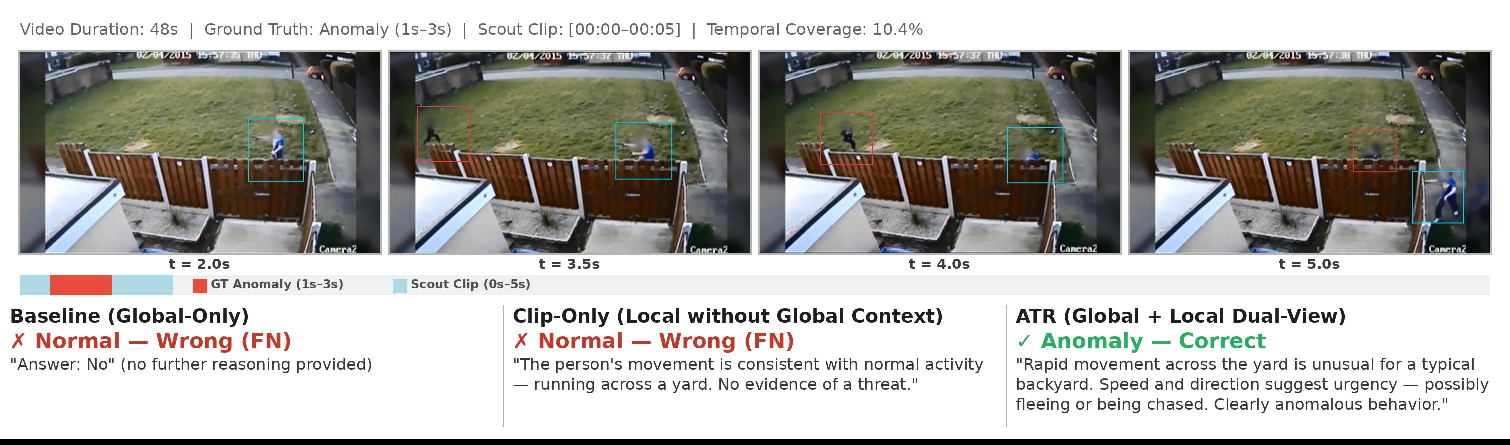
\includegraphics[width=\linewidth]{figures/fig_qualitative.pdf}
  \caption{Qualitative comparison on \emph{Shooting007}. ATR fuses global context (establishing the setting) with local detail (amplifying urgency cues), yielding a correct Anomaly classification where baselines fail.}
  \label{fig:qualitative}
\end{figure*}

\subsection{Cross-Paradigm Comparison}
\label{sec:cross_paradigm}

\begin{table}[t]
  \centering
  \caption{Cross-paradigm performance comparison on the UCF-Crime standard test set ($N$=290). ``--'' denotes an inapplicable metric. $\dagger$~LAVAD frame scores are max-aggregated per video and binarized with threshold $t$; $t{=}0.5$ is fixed, while oracle $t$ is selected post hoc on this evaluation set and is reported only as an upper-bound reference.}
  \label{tab:cross_paradigm}
  \resizebox{\columnwidth}{!}{%
  \begin{tabular}{lccccc}
    \toprule
    Method & Supervision & F.AUC$\uparrow$ & V.Acc$\uparrow$ & V.FNR$\downarrow$ & V.FPR$\downarrow$ \\
    \midrule
    LAVAD\textsuperscript{$\dagger$} ($t$=0.5)~\cite{zanella2024harnessing} & Training-Free & 80.28\% & 67.59\% & 63.57\% & 3.33\% \\
    LAVAD\textsuperscript{$\dagger$} (oracle $t$)~\cite{zanella2024harnessing} & Training-Free & 80.28\% & 82.76\% & 22.14\% & 12.67\% \\
    Gemini 3.1 Pro~\cite{team2023gemini} & Zero-Shot & -- & 73.10\% & 6.43\% & 46.00\% \\
    \textbf{ATR (Qwen3-VL-4B)} & \textbf{Zero-Shot} & -- & \textbf{85.17\%} & \textbf{11.43\%} & \textbf{18.00\%} \\
    \textbf{ATR (Qwen3-VL-8B)} & \textbf{Zero-Shot} & -- & \textbf{85.52\%} & \textbf{20.00\%} & \textbf{9.33\%} \\
    \bottomrule
  \end{tabular}}
\end{table}

Gemini 3.1 Pro obtains low FNR but a 46.00\% FPR under our zero-shot prompt, illustrating why accuracy, FNR, and FPR must be interpreted together. ATR's 4B and 8B operating points achieve higher accuracy with substantially lower FPR in this protocol. We do not mix these video-level results with weakly supervised frame-level SOTA rankings because the supervision, output granularity, and metrics differ.

\subsection{Cross-Dataset Generalization: XD-Violence}
\label{sec:xd_violence}

\begin{table}[t]
  \centering
  \caption{XD-Violence per-model best prompt: Baseline vs.\ ATR ($N$=800).}
  \label{tab:xd_best}
  \resizebox{\columnwidth}{!}{%
  \begin{tabular}{llcccccc}
    \toprule
    Model & Prompt & BL Acc & ATR Acc & $\Delta$ Acc & BL FNR & ATR FNR & $\Delta$ FNR \\
    \midrule
    4B & Minimal & 34.12\% & \textbf{49.00\%} & \textbf{+14.88\%} & 67.27\% & \textbf{48.53\%} & \textbf{$-$18.74\%} \\
    8B & Aggressive & 42.38\% & \textbf{50.75\%} & \textbf{+8.37\%} & 54.97\% & \textbf{46.57\%} & \textbf{$-$8.39\%} \\
    \bottomrule
  \end{tabular}}
\end{table}

Despite the lower absolute accuracy (a consequence of XD-Violence's heavy audio dependence, which disadvantages vision-only models), the relative improvement (+14.88\%) substantially exceeds that on UCF-Crime (+1.72\%), consistent with the greater headroom available when the baseline is weaker. This interpretation is further supported by the Qwen2.5-Omni experiment (Section~\ref{sec:omni}), where restoring the audio modality yields +29.33\% accuracy.


\subsection{Cross-Modal Validation: Qwen2.5-Omni on XD-Violence}
\label{sec:omni}

To further unlock ATR's potential through \textbf{spatio-temporal joint zoom-in}, we evaluate with Qwen2.5-Omni-7B~\cite{xu2025qwenomni} on XD-Violence. The global scan runs at 1~FPS while the Sniper clip runs at 2~FPS (Qwen2.5-Omni supports explicit frame-rate specification, unlike Qwen3-VL's duration-proportional allocation), producing a genuine physical frame-rate differential in addition to temporal window compression. Combined with native audio-visual joint reasoning, this activates all three amplification channels simultaneously.

\begin{table}[t]
  \centering
  \caption{Qwen2.5-Omni-7B on XD-Violence ($N$=800): 3 prompt styles.}
  \label{tab:omni}
  \resizebox{\columnwidth}{!}{%
  \begin{tabular}{lccccccc}
    \toprule
    Prompt & BL Acc & ATR Acc & $\Delta$ Acc & BL F1 & ATR F1 & BL FNR & ATR FNR \\
    \midrule
    \textbf{Minimal} & 38.42\% & \textbf{67.75\%} & \textbf{+29.33\%} & 53.50\% & \textbf{80.63\%} & 60.36\% & \textbf{24.90\%} \\
    Aggressive & 32.29\% & 54.44\% & +22.15\% & 47.83\% & 69.36\% & 65.27\% & 42.30\% \\
    Neutral & 28.54\% & 47.50\% & +18.96\% & 42.96\% & 62.16\% & 69.89\% & 51.75\% \\
    \bottomrule
  \end{tabular}}
\end{table}

Under full-modality conditions, Qwen2.5-Omni achieves substantial positive gains under \textbf{all three prompt styles} (+18.96\%--+29.33\% Accuracy), eliminating the prompt sensitivity observed in vision-only models. The Minimal configuration improves F1 from 53.50\% to 80.63\% (+27.13) and reduces FNR from 60.36\% to 24.90\% ($-$35.46\%). The larger gains compared to vision-only models (+29.33\% vs.\ +14.88\%) suggest that audio-visual joint reasoning provides a complementary amplification channel for ATR.


\subsection{Cross-Model-Family Validation: Qwen3.5-VL}
\label{sec:qwen35}

To evaluate whether ATR's observed patterns generalize beyond the Qwen3-VL family, we conduct experiments on the next-generation \textbf{Qwen3.5-VL-Instruct} series (9B and 27B) using the same UCF-Crime standard test set ($N$=290) and three prompt strategies. Thinking mode is disabled (\texttt{enable\_thinking=False}) to ensure outputs are directly comparable to Qwen3-VL experiments.

\begin{table}[t]
  \centering
  \caption{Qwen3.5-VL on UCF-Crime ($N$=290): Baseline vs.\ ATR.}
  \label{tab:qwen35}
  \resizebox{\columnwidth}{!}{%
  \begin{tabular}{llcccccc}
    \toprule
    Model & Prompt & BL Acc & ATR Acc & $\Delta$ Acc & BL FNR & ATR FNR & $\Delta$ FNR \\
    \midrule
    9B & Minimal & 86.90\% & 66.21\% & $-$20.69\% & 12.86\% & 30.00\% & +17.14\% \\
    9B & Aggressive & 81.72\% & 66.90\% & $-$14.83\% & 24.29\% & 11.43\% & $-$12.86\% \\
    9B & \textbf{Neutral} & 82.41\% & \textbf{85.52\%} & \textbf{+3.10\%} & 33.57\% & \textbf{21.43\%} & \textbf{$-$12.14\%} \\
    \midrule
    27B & Minimal & 85.17\% & 76.90\% & $-$8.28\% & 20.00\% & 31.43\% & +11.43\% \\
    27B & Aggressive & 84.48\% & 82.07\% & $-$2.41\% & 16.43\% & 19.29\% & +2.86\% \\
    27B & Neutral & 85.52\% & 83.45\% & $-$2.07\% & 14.29\% & 28.57\% & +14.28\% \\
    \bottomrule
  \end{tabular}}
\end{table}

Qwen3.5-9B achieves 86.90\% baseline accuracy (Minimal), already surpassing the best Qwen3-VL ATR result (8B+ATR, 85.52\%; Table~\ref{tab:cross_scale}). Only 9B+Neutral yields a positive ATR gain (+3.10\%); all other configurations show negative or marginal returns, consistent with the diminishing-returns pattern observed for Qwen3-VL~32B and analyzed in Section~\ref{sec:over_alignment}.

\subsection{Cross-Framework Validation: LLaVA-NeXT-Video}
\label{sec:llava_validation}

To test whether the observed gain is specific to the Qwen VLM interface, we evaluate LLaVA-NeXT-Video-7B-Qwen2 with a fixed aggressive prompt on the same UCF-Crime test set. Baseline and ATR use identical decoding and Yes/No parsing; the only protocol change is global-only input versus the full-video-plus-retrieved-clip Sniper input.

\begin{table}[t]
  \centering
  \caption{Cross-backbone check with LLaVA-NeXT-Video-7B-Qwen2 on UCF-Crime ($N$=290), using the same aggressive prompt for both methods.}
  \label{tab:llava_validation}
  \resizebox{\columnwidth}{!}{%
  \begin{tabular}{lcccccc}
    \toprule
    Method & Acc & Prec & Rec & F1 & FPR & FNR \\
    \midrule
    Global-Only & 72.76\% & 100.00\% & 43.57\% & 60.70\% & 0.00\% & 56.43\% \\
    \textbf{ATR} & \textbf{77.24\%} & 100.00\% & \textbf{52.86\%} & \textbf{69.16\%} & 0.00\% & \textbf{47.14\%} \\
    \bottomrule
  \end{tabular}}
\end{table}

ATR improves accuracy by 4.48 points and recall by 9.29 points without increasing FPR in this configuration. This matched-prompt comparison supports transfer of the input protocol beyond the main Qwen-VL implementation. The complete LLaVA-family sweep is mixed (Appendix Table~\ref{tab:llava_full}), so we describe ATR as framework-, backbone-, and alignment-sensitive rather than universally VLM-agnostic.
